
\documentclass[12pt,a4paper,landscape]{article}
\usepackage[latin1]{inputenc}
\usepackage{amsmath}
\usepackage{amsfonts}
\usepackage{amssymb}
\usepackage{graphicx}
\usepackage{lscape}
\usepackage{multicol}
\usepackage{setspace}
\usepackage[margin=2.5cm]{geometry}
\newcommand{\est}[2]{\begin{array}[t]{c}
\hspace{-.125in}#1\hspace{-.125in}\vspace{-.13in}\\ 
\hspace{-.125in}#2\hspace{-.125in}
\end{array}}
\linespread{1.6}
\newcommand{\arr}{  (\mathsf{1}   + \est{\mathsf{  0.00}}{(\mathsf{  0.07})} B + \est{\mathsf{  0.03}}{(\mathsf{  0.07})} B^{\mathsf{2}} - \est{\mathsf{  0.06}}{(\mathsf{  0.07})} B^{\mathsf{3}} - \est{\mathsf{  0.04}}{(\mathsf{  0.07})} B^{\mathsf{4}} - \est{\mathsf{  0.02}}{(\mathsf{  0.07})} B^{\mathsf{5}} - \est{\mathsf{  0.06}}{(\mathsf{  0.06})} B^{\mathsf{6}} - \est{\mathsf{  0.07}}{(\mathsf{  0.07})} B^{\mathsf{7}} - \est{\mathsf{  0.04}}{(\mathsf{  0.07})} B^{\mathsf{8}} - \est{\mathsf{  0.02}}{(\mathsf{  0.07})} B^{\mathsf{9}} - \est{\mathsf{  0.00}}{(\mathsf{  0.06})} B^{\mathsf{10}} + \est{\mathsf{  0.08}}{(\mathsf{  0.07})} B^{\mathsf{11}} - \est{\mathsf{  0.10}}{(\mathsf{  0.07})} B^{\mathsf{12}} + \est{\mathsf{  0.08}}{(\mathsf{  0.07})} B^{\mathsf{13}} - \est{\mathsf{  0.11}}{(\mathsf{  0.07})} B^{\mathsf{14}} + \est{\mathsf{  0.02}}{(\mathsf{  0.07})} B^{\mathsf{15}} + \est{\mathsf{  0.13}}{(\mathsf{  0.07})} B^{\mathsf{16}} + \est{\mathsf{  0.01}}{(\mathsf{  0.07})} B^{\mathsf{17}} + \est{\mathsf{  0.14}}{(\mathsf{  0.07})} B^{\mathsf{18}} ) }
\newcommand{\ifmu}{- \est{\mathsf{920.63}}  {(\mathsf{7.53})}} 
 \begin{document}
\begin{flushleft}
\thispagestyle{empty}
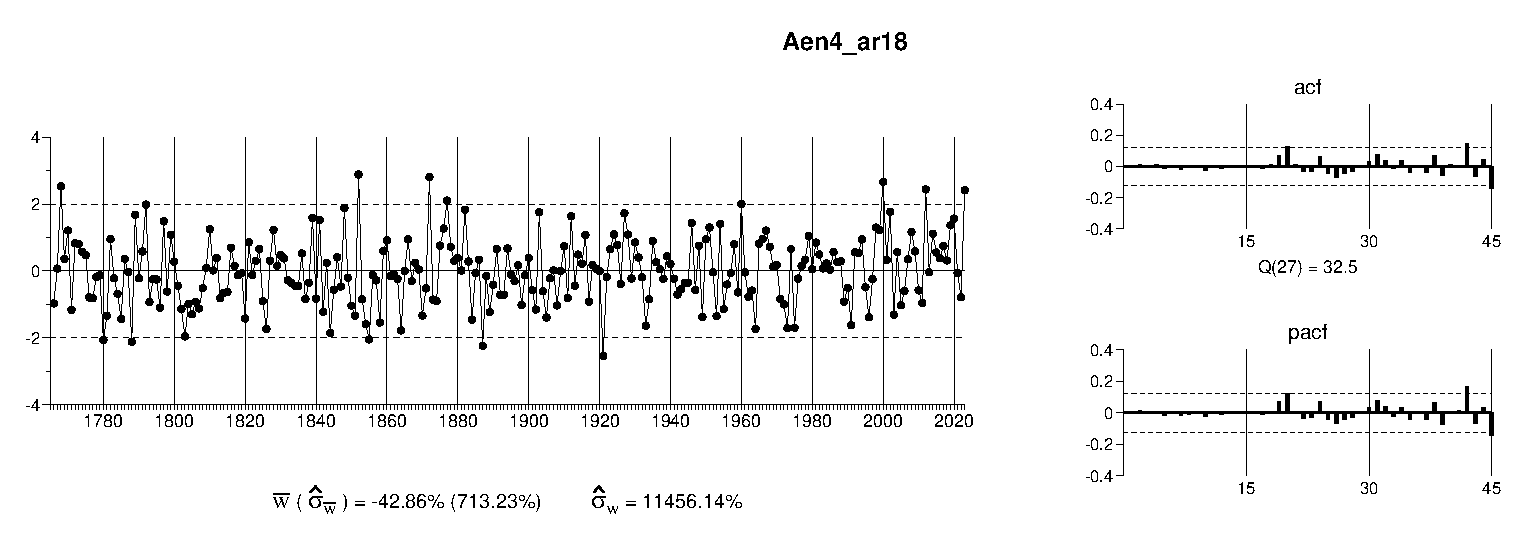
\includegraphics[scale=.90]{Aen4_ar18.eps}
\begin{footnotesize}
 $ \arr 
\left[ 
\mathsf{EN.1}_{t}\ifmu \right] 
 = \mathsf{Aen4_ar18_{t}} ; \quad 
\hat{\sigma}_{\mathsf{Aen4_ar18}}=  \mathsf{ 11497.67 } \%  $ 

\bigskip 
\begin{multicols}{2}{ 
\begin{tabular}{ccc}
\hline  Obs.  &  Date &  Std. Val. \\ 
\hline 
  & &  \vspace{-.12in} \\  
  & &  \vspace{-.12in} \\  
  & &  \vspace{-.12in} \\  
  & &  \vspace{-.12in} \\  
  & &  \vspace{-.12in} \\  
  & &  \vspace{-.12in} \\  
  & &  \vspace{-.12in} \\  
  & &  \vspace{-.12in} \\  
  & &  \vspace{-.12in} \\  
  & &  \vspace{-.12in} \\  
  & &  \vspace{-.12in} \\  
  & &  \vspace{-.12in} \\  
  & &  \vspace{-.12in} \\  
  & &  \vspace{-.12in} \\  
  & &  \vspace{-.12in} \\  
  & &  \vspace{-.12in} \\  
  & &  \vspace{-.12in} \\  
  & &  \vspace{-.12in} \\  
  & &  \vspace{-.12in} \\  
  & &  \vspace{-.12in} \\  
  & &  \vspace{-.12in} \\  
  & &  \vspace{-.12in} \\  
 \end{tabular} 
\\ 
 \columnbreak 
 \singlespacing 
 \underline{\textbf{Comments:}} \\ 
 \bigskip       

% \underline{Action:} 
 } 
\end{multicols} 

\end{footnotesize}
\end{flushleft}
\end{document}
